\chapter{Bài 3. Đơn vị và sai số trong vật lí}
\begin{center}
	\textit{(3 tiết)}
\end{center}
\section{MỤC TIÊU DẠY HỌC}
\begin{center}
	\begin{longtable}{|M{2.5cm}|L{12.5cm}|M{2cm}|}
		\hline
		\thead{Biểu hiện\\ năng lực} & \thead{Mục tiêu} & \thead{STT}\\
		\hline
		\multicolumn{3}{|c|}{\textbf{ Năng lực vật lí}}\\
		\hline
		1.1 & Nêu được hệ đơn vị SI, đơn vị cơ bản, đơn vị dẫn xuất & 1\\
		\hline
		1.1& Nêu được khái niệm thứ nguyên & 2\\
		\hline
		1.2 & Vận dụng được mối liên hệ giữa đơn vị dẫn xuất với 7 đơn vị cơ bản &3\\
		\hline
		1.1 & Thảo luận để nêu được một số loại sai số đơn giản hay gặp khi đo các đại lượng vật lí và cách khắc phục chúng & 4\\
		\hline
		1.2 & Biểu diễn được kết quả đo đại lượng vật lí & 5\\
		\hline
		1.2 & Xác định được sai số trong phép đo gián tiếp & 6\\
		\hline
		\multicolumn{3}{|c|}{\textbf{Năng lực chung}}\\
		\hline
		TC - TH& Tích cực thực hiện các nhiệm vụ GV đặt ra cho các nhóm, tích cực suy luận để đưa ra câu trả lời trong quá trình GV định hướng nội dung học tập	&7 \\
		\hline
		GT - HT & Tích cực đóng góp ý kiến trong quá trình thảo luận, biết sử dụng ngôn ngữ kết hợp với các loại phương tiện phi ngôn ngữ đa dạng để trình bày các kết quả thảo luận nhóm & 8\\
		\hline
	\end{longtable}
\end{center}
\section{THIẾT BỊ DẠY HỌC VÀ HỌC LIỆU}
\begin{itemize}
	\item Tivi/máy chiếu;
	\item SGK;
	\item Phiếu học tập.
\end{itemize}
\section{TIẾN TRÌNH DẠY HỌC}
\subsection{TIẾN TRÌNH}\newpage
\begin{center}
	\begin{longtable}{|L{2.75cm}|C{1.25cm}|L{5cm}|L{3.5cm}|L{4cm}|}
		\hline
		\thead{Tiến trình} & \thead{Mục\\tiêu} & \thead{Nội dung dạy học \\trọng tâm} & \thead{PP,\\ KTDH} & \thead{Phương pháp \\đánh giá}\\
		\hline
		\textbf{Hoạt động 1:} Tìm hiểu đơn vị và thứ nguyên trong vật lí&1, 2  & Hệ đơn vị SI, đơn vị cơ bản và đơn vị dẫn xuất, thứ nguyên  & PP: Đàm thoại\newline
		KTDH: Kĩ thuật "tia chớp"  & GV đánh giá dựa trên câu trả lời của HS.\newline
		PP đánh giá: quan sát, nghe. \\
		\hline
		\textbf{Hoạt động 2:} Vận dụng mối liên hệ giữa đơn vị dẫn xuất và đơn vị cơ bản & 3, 7, 8 & Mối liên hệ giữa đơn vị dẫn xuất và đơn vị cơ bản & PP: Dạy học hợp tác\newline
		KTDH: Kĩ thuật "các mảnh ghép" & GV đánh giá dựa trên thái độ của HS trong các nhóm và kết quả thảo luận nhóm.\newline PP đánh giá: quan sát, nghe.\\
		\hline
		\textbf{Hoạt động 3:} Tìm hiểu sai số trong phép đo và cách hạn chế & 4, 7, 8 & Các phép đo, các loại sai số trong vật lí & PP: Dạy học hợp tác.\newline
		KTDH: Đọc tích cực, chia sẻ cặp đôi & GV đánh giá dựa trên câu trả và phiếu học tập nhóm đôi của HS.\newline PP đánh giá: quan sát, nghe.\\
		\hline
		\textbf{Hoạt động 4:} Tìm hiểu cách biểu diễn sai số của phép đo & 5, 6, 7, 8 & Cách biểu diễn kết quả đo trực tiếp, cách xác định sai số trong phép đo gián tiếp & PP: Đàm thoại.\newline KTDH: kĩ thuật "chia sẻ cặp đôi" & GV đánh giá dựa trên phiếu học tập của HS.\newline
		PP đánh giá: quan sát, nghe.\\
		\hline
		\textbf{Hoạt động 5:} Luyện tập & 1 - 6 & Luyện tập bài tập xác định CSCN, xác định sai số trong phép đo trực tiếp, sai số trong phép đo gián tiếp & PP: Đàm thoại. & GV đánh giá dựa trên bài tập cá nhân của HS\newline
		PP đánh giá: quan sát, nghe.\\
		\hline
	\end{longtable}
\end{center}
\subsection{CÁC HOẠT ĐỘNG HỌC}
\hoatdong{Tìm hiểu đơn vị và thứ nguyên trong vật lí
}
{
HS nêu được hệ đơn vị SI, đơn vị cơ bản và đơn vị dẫn xuất.

HS nêu được thứ nguyên của các đại lượng vật lí, phân biệt được thứ nguyên với đơn vị.
}
{
Câu trả lời của HS.
}
{
\textit{\underline{* GV chuyển giao nhiệm vụ học tập}}\\
GV dẫn dắt vào bài. GV sử dụng kĩ thuật "tia chớp" yêu cầu HS kể tên một số đại lượng vật lí và đơn vị của chúng mà HS đã được học trong môn KHTN.\\
GV giới thiệu về hệ đơn vị SI, các đơn vị cơ bản, tên và kí hiệu tiếp đầu ngữ của bội số, ước số thập phân của đơn vị.\\
GV giới thiệu khái niệm thứ nguyên, cách xác định thứ nguyên của đại lượng vật lí, nguyên tắc về thứ nguyên trong 1 biểu thức vật lí.\\
GV lấy ví dụ hướng dẫn học sinh xác định thứ nguyên của tốc độ.\\
\textit{\underline{* HS thực hiện nhiệm vụ học tập}}\\
HS tích cực trả lời câu hỏi gợi mở của GV.\\
HS chú ý theo dõi, đặt câu hỏi.\\
\textit{\underline{* HS báo cáo kết quả nhiệm vụ học tập}}
\begin{itemize}[label=-]
	\item GV lần lượt mời HS trả lời câu hỏi.
	\item Các HS khác theo dõi và nhận xét.
	\item GV nhận xét và chuẩn hóa kiến thức.
\end{itemize}
}
% ===============================================================
\hoatdong{Vận dụng mối liên hệ giữa đơn vị dẫn xuất và đơn vị cơ bản}
{
HS vận dụng được mối liên hệ giữa đơn vị dẫn xuất với 7 đơn vị cơ bản của hệ SI.
}
{
Phiếu học tập 1.
}
{\textit{\underline{* GV chuyển giao nhiệm vụ học tập}}\\
	GV hướng dẫn HS thực hiện ví dụ trong SGK trang 17 mục "Vận dụng mối liên hệ giữa đơn vị dẫn xuất với 7 đơn vị cơ bản của hệ SI".\\
	GV sử dụng kĩ thuật "các mảnh ghép" cho HS thực hiện hoạt động học tập 2:
	\begin{itemize}
		\item \textbf{Vòng 1:} GV chia lớp thành 6 nhóm, mỗi nhóm gồm  2 bàn quay lại với nhau. GV phân công nhóm 1 + 4 thực hiện nhiệm vụ 1; nhóm 2 + 5 thực hiện nhiệm vụ 2; nhóm 3 + 6 thực hiện nhiệm vụ 3 trong phiếu học tập 1. GV yêu cầu các nhóm thảo luận tích cực và đảm bảo mỗi thành viên đều nắm được kết quả thảo luận của nhóm. Trong mỗi nhóm, GV đánh STT các thành viên từ 1 đến 6. Hoạt động vòng 1 diễn ra trong 10 phút. Các nhóm ghi lại kết quả thảo luận vào phiếu học tập của nhóm để nộp lại cho GV.
		\item \textbf{Vòng 2:} GV yêu cầu các HS có cùng STT di chuyển về 1 nhóm. Các HS lần lượt trao đổi với các thành viên còn lại trong nhóm về kết quả thảo luận ở vòng 1. Các nhóm thảo luận tích cực và đảm bảo rằng các thành viên trong nhóm đều nắm được kết quả của 3 nhiệm vụ học tập. Các nhóm thống nhất trình bày kết quả 3 nhiệm vụ vào biên bản chung để nộp cho GV. Hoạt động vòng 2 diễn ra trong 15 phút.
	\end{itemize}
\textit{\underline{* HS thực hiện nhiệm vụ học tập}}\\
HS hoạt động theo nhóm được phân công, tích cực thảo luận.\\
Trong quá trình di chuyển, HS trật tự và đi theo hướng dẫn của GV.\\
\textit{\underline{* HS báo cáo kết quả thực hiện nhiệm vụ học tập}}\\
GV chọn đại diện của 3 nhóm HS bất kì lên bảng trình bày kết quả thảo luận.\\
HS chú ý theo dõi, nhận xét phần trình bày của các nhóm.\\
GV chỉnh lí, hợp thức hoá kiến thức.

}
% ========================================================
\hoatdong{
	Tìm hiểu sai số trong phép đo và cách hạn chế
}
{
	HS nêu được một số loại sai số đơn giản hay gặp khi đo các đại lượng vật lí.\\
	HS nêu được giải pháp hạn chế một số loại sai số đơn giản hay gặp khi đo các đại lượng vật lí.
}
{
Phiếu học tập 2
}
{\textit{\underline{* GV chuyển giao nhiệm vụ học tập}}\\
	GV yêu cầu HS hoạt động theo nhóm 2 hoặc nhóm 3 HS.\\
	GV yêu cầu các nhóm nghiên cứu SGK mục "Các phép đo trong vật lí" và "Các loại sai số của phép đo" để hoàn thành 2 bảng so sánh trong phiếu học tập 2.\\
	\textit{\underline{* HS thực hiện nhiệm vụ học tập}}\\
	HS hoạt động theo nhóm được chia, đọc tích cực và hoàn thành bảng so sánh ở phiếu học tập 2.\\
	GV theo dõi hoạt động của các nhóm, hỗ trợ khi HS gặp khó khăn.\\
	\textit{\underline{* HS báo cáo kết quả thực hiện nhiệm vụ học tập}}\\
	GV lần lượt mời các nhóm bất kì điền kết quả vào bảng so sánh.\\
	HS theo dõi, nhận xét, đặt câu hỏi.\\
	GV chỉnh lí, hợp thức hoá kiến thức.

}
% ===========================================================
\hoatdong{
Tìm hiểu cách biểu diễn sai số của phép đo
}
{
HS xác định được sai số trong phép đo trực tiếp và phép đo gián tiếp.\\
HS biểu diễn được kết quả đo đại lượng vật lí.
}
{Bài tập vận dụng xác định sai số trong phép đo trực tiếp và sai số trong phép đo gián tiếp

}
{\textit{\underline{* GV chuyển giao nhiệm vụ học tập}}\\
	GV giới thiệu cho HS các khái niệm: giá trị trung bình, sai số tuyệt đối, sai số tương đối.\\
	GV hướng dẫn HS cách biểu diễn sai số của phép đo trực tiếp, cách xác định số CSCN và quy tắc làm tròn số.\\
	GV dẫn dắt cho HS làm bài tập vận dụng 1 ở Bảng 3.4 SGK CTST trang 22.\\
	GV hướng dẫn HS cách xác định sai số gián tiếp.\\
	GV dẫn dắt HS thực hiện bài tập vận dụng 2 trang 22.\\
	\textit{\underline{* HS thực hiện nhiệm vụ học tập}}\\
	HS chú ý lắng nghe phần hướng dẫn của GV và đặt câu hỏi (nếu có).\\
	HS thực hiện bài tập vận dụng 1 và vận dụng 2.\\
	\textit{\underline{* HS báo cáo kết quả thực hiện nhiệm vụ học tập}}\\
	GV mời HS trả lời trong quá trình hướng dẫn bài tập vận dụng 1 và vận dụng 2.\\
	GV chỉnh lí, hợp thức hoá kiến thức.
}
%%%%%%%%%%%%%%%%%%%%%%%%%%%%%%%%%%%%%%%%%%%%%
\hoatdong{
	Luyện tập.
}
{
	HS xác định được số CSCN, sai số trong phép đo trực tiếp, sai số trong phép đo gián tiếp.
}
{
	Bài tập cá nhân của học sinh.
}
{
	\textit{\underline{* GV chuyển giao nhiệm vụ học tập}}\\
	GV lần lượt chuyển giao từng bài tập, yêu cầu HS hoạt động cá nhân để giải.\\
	\textit{\underline{* HS thực hiện nhiệm vụ học tập}}\\
	HS \textit{(làm việc cá nhân)}:  Giải bài tập trong phiếu bài tập được GV giao. 
	
	GV: Theo dõi để phát hiện các HS gặp khó khăn, từ đó đưa ra sự định hướng, hỗ trợ phù hợp cho mỗi HS.\\
	\textit{\underline{* HS báo cáo kết quả thực hiện nhiệm vụ học tập}}\\
	GV: Mời HS lên bảng giải bài tập.
	
	HS: Đặt câu hỏi, góp ý.
	
	GV: Chỉnh lí, hợp thức hoá kiến thức.
}

\section{HỒ SƠ DẠY HỌC}
\subsection{NỘI DUNG DẠY HỌC}
\begin{enumerate}[label=\bfseries\Roman*.]
	\item \textbf{ĐƠN VỊ VÀ THỨ NGUYÊN TRONG VẬT LÍ}\\
	Trong khoa học có rất nhiều hệ đơn vị được sử dụng, trong đó thông dụng nhất là hệ đơn vị đo lường quốc tế SI (Système International d’unités) được xây dựng trên cơ sở của 7 đơn vị cơ
	bản.
	\begin{enumerate}[label=\bfseries\arabic*.]
		\item \textbf{Các đơn vị cơ bản trong hệ SI}
		\begin{center}
			\begin{longtable}{|M{1.5cm}|M{3cm}|M{3cm}|M{4cm}|}
				\hline
				\thead{STT}&\thead{Đơn vị}& \thead{Kí hiệu} &\thead{Đại lượng}\\
				\hline
				1 & mét & $\si{\meter}$ & Chiều dài\\
				\hline
				2 & kilogram & $\si{\kilogram}$ & Khối lượng \\
				\hline
				3 & giây & $\si{\second}$ & Thời gian \\
				\hline
				4 & kelvin & $\si{\kelvin}$ & Nhiệt độ \\
				\hline
				5 & ampere & $\si{\ampere}$ & Cường độ dòng điện\\
				\hline
				6 & mol & $\si{\mole}$ & Lượng chất\\
				\hline
				7 & candela & $\si{\candela}$ &  Cường độ sáng\\
				\hline
			\end{longtable}
		\end{center}
	Ngoài 7 đơn vị cơ bản, những đơn vị còn lại được gọi là \textbf{đơn vị dẫn xuất}.
	\item \textbf{Tên và kí hiệu tiếp đầu ngữ của bội số, ước số thập phân của đơn vị}
	\begin{center}
		\newcolumntype{a}[1]{>{\centering\arraybackslash\columncolor{gray}}p{#1}}
		\begin{longtable}{|M{2cm}|M{2cm}|M{2cm}|a{0.5cm}|M{2cm}|M{2cm}|M{2cm}|}
			\hline
			\thead{Kí hiệu}&\thead{Tên đọc}& \thead{Hệ số}&&\thead{Kí hiệu}&\thead{Tên đọc}&\thead{Hệ số}\\
			\hline
			Y &yotta& $10^{24}$&&y & yokto &$10^{-24}$\\ 
			\hline
			Z &zetta& $10^{21}$&&z & zepto &$10^{-21}$\\ 
			\hline
			E &eta& $10^{18}$&&a & atto &$10^{-18}$\\ 
			\hline
			P &peta& $10^{15}$&&f & femto &$10^{-15}$\\ 
			\hline
			T &tera& $10^{12}$&&p & pico &$10^{-12}$\\ 
			\hline
			G &giga& $10^{9}$&&n & nano &$10^{-9}$\\ 
			\hline
			M &mega& $10^{6}$&&$\mathnormal{\mu}$ & micro &$10^{-6}$\\ 
			\hline
			k &kilo& $10^{3}$&&m & milli &$10^{-3}$\\ 
			\hline
			h &hecto& $10^{2}$&&c & centi &$10^{-2}$\\ 
			\hline
			da &deka& $10^{1}$&&d & deci &$10^{-1}$\\ 
			\hline
		\end{longtable}
	\end{center}
\item \textbf{Thứ nguyên}\\
Thứ nguyên của một đại lượng là quy luật nêu lên sự phụ thuộc của đơn vị đo đại lượng đó vào các đơn vị cơ bản. Thứ nguyên của một đại lượng X được biểu diễn dưới dạng $\left[X\right]$.\\
\textbf{Thứ nguyên của một số đại lượng cơ bản}:
\begin{center}
	\begin{longtable}{|M{6cm}|M{6cm}|}
		\hline
		\thead{Đại lượng cơ bản}&\thead{Thứ nguyên}\\
		\hline
		[Chiều dài] & L\\
		\hline
		[Khối lượng] & M\\
		\hline
		[Thời gian] & T\\
		\hline
		[Cường độ dòng điện] & I\\
		\hline
		[Nhiệt độ]&K\\
		\hline
	\end{longtable}
\end{center}
\textbf{Ví dụ:} Tọa độ, quãng đường có thứ nguyên là L; vận tốc có thứ nguyên là $L\cdot T^{-1}$; khối lượng riêng có thứ nguyên là $M\cdot L^{-3}$,\dots\\
\textbf{Lưu ý:} Trong các biểu thức vật lí:
\begin{itemize}
	\item Các số hạng trong phép cộng (hoặc trừ) phải có cùng thứ
	nguyên.
	\item Hai vế của một biểu thức vật lí phải có cùng thứ nguyên.
\end{itemize}
\item \textbf{SAI SỐ TRONG PHÉP ĐO VÀ CÁCH HẠN CHẾ}\\
\begin{enumerate}[label=\bfseries\arabic*.]
	\item \textbf{Các phép đo trong vật lí}
	\begin{itemize}
		\item Phép đo các đại lượng vật lí là phép so sánh chúng với đại lượng cùng loại được quy ước làm đơn vị.
		\item \textit{Phép đo trực tiếp}: giá trị của đại lượng cần đo được đọc trực tiếp trên dụng cụ đo (ví dụ như đo khối lượng bằng cân, đo thể tích bằng bình chia độ).
		\item \textit{Phép đo gián tiếp}: giá trị của đại lượng cần đo được xác định thông qua các đại lượng được đo trực tiếp (ví dụ như đo khối lượng riêng).
	\end{itemize}
\item \textbf{Các loại sai số của phép đo}\\
\begin{enumerate}[label=\bfseries\alph*)]
	\item \textbf{Sai số hệ thống:} là sai số có tính quy luật và được lặp lại ở tất cả các lần đo. Sai số hệ thống làm cho giá trị đo tăng hoặc giảm một lượng nhất định so với giá trị thực.\\
	Sai số hệ thống thường xuất phát từ dụng cụ đo (ví dụ: không
	hiệu chỉnh dụng cụ về đúng số 0, \dots). Ngoài ra sai số hệ thống còn xuất phát từ độ chia nhỏ nhất của dụng cụ đo (gọi là sai số dụng cụ, thường được xác định bằng một nửa độ chia nhỏ nhất).\\
	$\Rightarrow$ Sai số hệ thống có thể hạn chế bằng cách hiệu chỉnh dụng cụ trước khi đo, lựa chọn dụng cụ đo phù hợp, thao tác đo đúng cách.
	\item \textbf{Sai số ngẫu nhiên:} là sai số xuất phát từ sai sót, phản xạ của người làm thí nghiệm hoặc từ những yếu tố ngẫu nhiên bên ngoài. Sai số này thường có nguyên nhân không rõ ràng và dẫn đến sự phân tán của các kết quả đo xung quanh một giá trị trung bình.\\
	Sai số ngẫu nhiên có thể được hạn chế bằng cách: thực hiện phép đo nhiều lần và lấy giá trị trung bình để hạn chế sự phân tán
	của số liệu đo.
\end{enumerate}
\item \textbf{Cách biểu diễn sai số của phép đo}\\
Khi tiến hành đo đạc, giá trị $x$ của một đại lượng vật lí thường được ghi dưới dạng
$$x=\overline{x}+\Delta x$$
với $\overline{x}$ là giá trị trung bình của đại lượng cần đo khi tiến hành phép đo nhiều lần:
$$\overline{x}=\dfrac{x_1+x_2+\dots+x_n}{n}$$
Sai số của phép đo được biểu diễn dưới dạng:
\begin{itemize}
	\item \textbf{Sai số tuyệt đối} $\Delta x$:
	\begin{itemize}
		\item Sai số tuyệt đối ứng với mỗi lần đo được xác định bằng trị tuyệt đối của hiệu giữa giá trị trung bình và giá trị của mỗi lần đo
		$$\Delta x_i=\left|\overline{x}-x_i\right|$$
		với $x_i$ là giá trị lần đo thứ $i$.
		\item Sai số tuyệt đối trung bình của $n$ lần đo được xác định theo công thức
		$$\overline{\Delta x}=\dfrac{\Delta x_1+\Delta x_2+\dots+\Delta x_n}{n}$$
		\item Sai số tuyệt đối của phép đo cho biết phạm vi biến thiên của giá trị đo được và bằng tổng của sai số ngẫu nhiên và sai số dụng cụ:
		$$\Delta x=\overline{\Delta x}+\Delta x_{\text{dc}}$$
		Trong đó sai số dụng cụ $\Delta x_{\text{dc}}$ thường được xem có giá trị bằng một nửa độ chia nhỏ nhất với những dụng cụ đơn giản như thước kẻ, cân bàn, bình chia độ, \dots
	\end{itemize}
\item \textbf{Sai số tương đối:} được xác định bằng tỉ số giữa sai số tuyệt đối và giá trị trung bình của đại lượng cần đo theo công thức:
$$\delta x=\dfrac{\Delta x}{\overline{x}}\cdot\SI{100}{\percent}$$
Sai số tương đối cho biết mức độ chính xác của phép đo.
\end{itemize}
\item \textbf{Cách xác định sai số trong phép đo gián tiếp}\\
Nguyên tắc xác định sai số trong phép đo gián tiếp như sau:
\begin{itemize}
	\item Sai số tuyệt đối của một tổng hay hiệu bằng tổng sai số tuyệt đối của các số hạng:\\
	Nếu $F=x\pm y\pm z\pm\dots$ thì $\Delta F=\Delta x+\Delta y+\Delta z+\dots$
	\item Sai số tương đối của một tích hoặc thương bằng tổng sai số tương đối của các thừa số:\\
	Nếu $F=x^m\dfrac{y^n}{z^k}$ thì $\delta F=m\cdot\delta x+n\cdot\delta y+k\cdot\delta z$.\\
	\textbf{\textit{Các chữ số có nghĩa gồm:}} Các chữ số khác 0, các chữ số 0 nằm giữa hai chữ số khác 0 hoặc nằm bên phải của dấu thập phân và một chữ số khác 0.\\
	\textbf{Ví dụ:} 765 có ba chữ số có nghĩa, 7005 có bốn chữ số có nghĩa, 0,0700 có ba chữ số có nghĩa.
\end{itemize}
\end{enumerate}

	\end{enumerate}
\end{enumerate}
\subsection{CÁC HỒ SƠ KHÁC}
\newpage
* Phiếu học tập 1
\begin{center}
	\begin{longtable}{|M{8.5cm}|M{8.5cm}|}
		\hline
		\multicolumn{2}{|c|}{\thead{PHIẾU HỌC TẬP  \\	VẬN DỤNG MỐI LIÊN HỆ GIỮA ĐƠN VỊ DẪN XUẤT VÀ ĐƠN VỊ CƠ BẢN
		}}\\
		\hline
		\multicolumn{1}{|L{8.5cm}}{Lớp: \dotfill} & \multicolumn{1}{L{8.5cm}|}{Nhóm: \dotfill}\\
		\multicolumn{2}{|L{17cm}|}{Tên: \dotfill}\\
		\hline
		\multicolumn{2}{|L{17cm}|}{\textbf{Nhiệm vụ 1:} Em hãy phân tích thứ nguyên của các đại lượng vật lí sau đây\newline
	\textit{* Gợi ý: Thứ nguyên của lực là $M\cdot L\cdot T^{-2}$.}	
	}\\
		\multicolumn{2}{|M{17cm}|}{
	\begin{center}
		\begin{tabular}{|M{8cm}|M{8cm}|}
			\hline
			\thead{Đại lượng} & \thead{Thứ nguyên}\\
			\hline
			Khối lượng riêng & \\
			\hline
			Công & \\
			\hline
			Công suất &\\
			\hline
			Áp suất & \\
			\hline
		\end{tabular}
	\end{center}	
	}\\
\hline
\multicolumn{
2
}{|L{17cm}|}{\textbf{Nhiệm vụ 2:} Tốc độ truyền sóng $v$ trên một sợi dây đàn hồi phụ thuộc vào lực căng $F$ và mật độ khối lượng $\mu$ (khối lượng trên một đơn vị chiều dài) của sợi dây. Bằng việc phân tích thứ nguyên, một bạn học sinh thiết lập biểu thức $v$ theo $F$ và $\mu$ như sau:
$$v=\alpha\cdot\dfrac{F}{\mu}$$
với $\alpha$ là hằng số không thứ nguyên. Công thức bạn học sinh đưa ra có phù hợp nguyên tắc thứ nguyên không?\newline
\textit{* Gợi ý: Thứ nguyên của lực là $M\cdot L\cdot T^{-2}$.}	
}\\
\multicolumn{2}{|L{17cm}|}{\dotfill}\\
\multicolumn{2}{|L{17cm}|}{\dotfill}\\
\multicolumn{2}{|L{17cm}|}{\dotfill}\\
\multicolumn{2}{|L{17cm}|}{\dotfill}\\
\multicolumn{2}{|L{17cm}|}{\dotfill}\\
\multicolumn{2}{|L{17cm}|}{\dotfill}\\
\hline
\multicolumn{2}{|L{17cm}|}{\textbf{Nhiệm vụ 3:} Lực cản không khí tác dụng lên vật phụ thuộc vào tốc độ chuyển động của vật theo công thức $F=-kv^2$. Biết thứ nguyên của lực là $M\cdot L\cdot T^{-2}$. Xác định thứ nguyên và đơn vị của $k$ trong hệ SI.
}\\
\multicolumn{2}{|L{17cm}|}{\dotfill}\\
\multicolumn{2}{|L{17cm}|}{\dotfill}\\
\multicolumn{2}{|L{17cm}|}{\dotfill}\\
\multicolumn{2}{|L{17cm}|}{\dotfill}\\
\multicolumn{2}{|L{17cm}|}{\dotfill}\\
\multicolumn{2}{|L{17cm}|}{\dotfill}\\
\hline
	\end{longtable}
\end{center}
\newpage
* Bảng quy đổi điểm hoạt động 2
\begin{center}
	\begin{longtable}{|M{2cm}|M{4cm}|M{4.5cm}|M{4cm}|M{2cm}|}
		\hline
		& \thead{Thái độ\\thảo luận}\newline \textit{(Tối đa 2,0 điểm)}& \thead{Số lượng\\ thành viên tích cực}\newline \textit{(Tối đa 2,0 điểm)} & \thead{Kết quả\\ thảo luận}\newline \textit{(Tối đa 6,0 điểm)} & \thead{Tổng\\ điểm}\\
		\hline
		\thead{Vòng 1} &&&&\\
		\hline
		\thead{Vòng 2} &&&&\\
		\hline
		\multicolumn{4}{|c|}{\cellcolor{gray!20!white}\color{red}\bfseries $\text{Tổng điểm} = \SI{40}{\percent}\times\text{Điểm vòng 1}+\SI{60}{\percent}\times\text{Điểm vòng 2}$}&\\
		\hline
	\end{longtable}
\end{center}
\newpage
* Phiếu học tập 2
\begin{center}
	\begin{longtable}{|M{8.5cm}|M{8.5cm}|}
		\hline
		\multicolumn{2}{|c|}{\thead{PHIẾU HỌC TẬP SỐ 2 \\	TÌM HIỂU CÁC LOẠI SAI SỐ TRONG PHÉP ĐO
		}}\\
		\hline
		\multicolumn{1}{|L{8.5cm}}{Lớp: \dotfill} & \multicolumn{1}{L{8.5cm}|}{Nhóm: \dotfill}\\
		\multicolumn{2}{|L{17cm}|}{Tên: \dotfill}\\
		\hline
		\multicolumn{2}{|L{17cm}|}{\textbf{Nhiệm vụ 1:} Em hãy phân biệt phép đo trực tiếp và phép đo gián tiếp, đưa ra ít nhất 2 ví dụ cho mỗi phép đo.
		}\\
		\multicolumn{2}{|M{17cm}|}{
			\begin{center}
				\begin{tabular}{|M{8cm}|M{8cm}|}
					\hline
					\thead{Phép đo trực tiếp} & \thead{Phép đo gián tiếp}\\
					\hline
				\dotfill&\dotfill\\
				\dotfill&\dotfill\\
				\dotfill&\dotfill\\
				\dotfill&\dotfill\\
					\hline
				\end{tabular}
			\end{center}	
		}\\
	\hline
	\multicolumn{2}{|L{17cm}|}{\textbf{Nhiệm vụ 2:} Em hãy phân biệt sai số hệ thống và sai số ngẫu nhiên theo các tiêu chí ở bảng bên dưới.
	\begin{center}
		\begin{tabular}{|L{3cm}|M{6cm}|M{6cm}|}
			\hline
			&\thead{Sai số hệ thống} & \thead{Sai số ngẫu nhiên}\\
			\hline
			Đặc điểm & & \vspace{4em}\\
			\hline
			Nguyên nhân & & \vspace{4em}\\
			\hline
			Cách hạn chế & & \vspace{4em}\\
			\hline
		\end{tabular}
	\end{center}	
}\\
\hline
\multicolumn{2}{|L{17cm}|}{\textbf{Nhiệm vụ 3:} Em hãy xác định nguyên nhân gây ra sai số khi đo trong các trường hợp dưới đây.
\begin{center}
	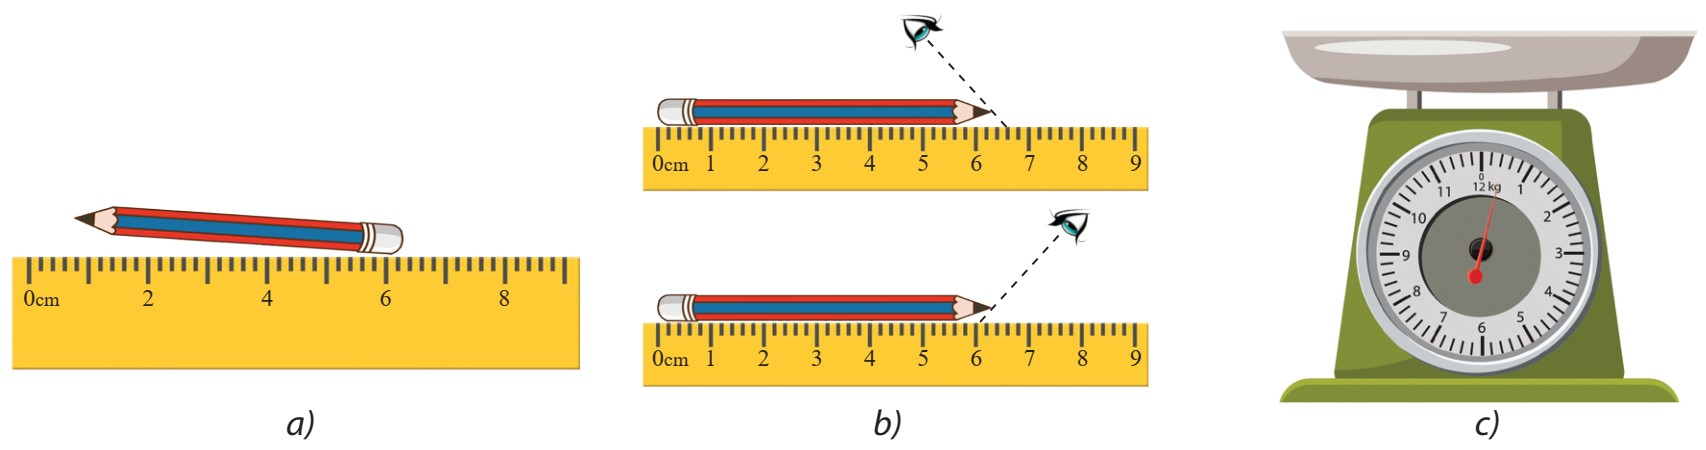
\includegraphics[width=0.7\linewidth]{figs/BAI3-1}
\end{center}

}\\
\multicolumn{2}{|L{17cm}|}{\dotfill
}\\
\hline
\end{longtable}
\end{center}
* Bài tập vận dụng 
% ======================================================================
\begin{ex}
Bảng bên dưới thể hiện	kết quả đo khối lượng của một túi trái cây bằng cân đồng hồ. Em hãy xác định sai số tuyệt đối ứng với từng lần đo, sai số tuyệt đối và sai số tương đối của phép đo. Biết sai số dụng cụ là $\SI{0.1}{\kilogram}$.
\begin{center}
	\begin{longtable}{|M{5.5cm}|M{5.5cm}|M{5.5cm}|}
		\hline
		\thead{Lần đo} & $\xsi{m}{\left(\kilogram\right)}$ & $\xsi{\Delta m}{\left(\kilogram\right)}$\\
		\hline
		1 & 4,2 &\\
		\hline
		2 & 4,4 &\\
		\hline
		3 & 4,4 &\\
		\hline
		4 & 4,2 &\\
		\hline
		\thead{Trung bình}&$\overline{m}=$ &$\overline{\Delta m}=$\\
		\hline
	\end{longtable}
\end{center}
Sai số tuyệt đối của phép đo: $\Delta m=\overline{\Delta m}+\Delta m_{\text{dc}}=$ \dotfill\\
Sai số tương đối của phép đo: $\delta m=\dfrac{\Delta m}{\overline{m}}\cdot\SI{100}{\percent}=$ \dotfill\\
Kết quả phép đo: $m=\overline{m}\pm\Delta m=$ \dotfill
	\loigiai{
\begin{center}
	\begin{longtable}{|M{5.5cm}|M{5.5cm}|M{5.5cm}|}
		\hline
		\thead{Lần đo} & $\xsi{m}{\left(\kilogram\right)}$ & $\xsi{\Delta m}{\left(\kilogram\right)}$\\
		\hline
		1 & 4,2 &0,1\\
		\hline
		2 & 4,4 &0,1\\
		\hline
		3 & 4,4 &0,1\\
		\hline
		4 & 4,2 &0,1\\
		\hline
		\thead{Trung bình}&$\overline{m}=4,3$ &$\overline{\Delta m}=0,1$\\
		\hline
	\end{longtable}
\end{center}
Sai số tuyệt đối của phép đo: $\Delta m=\overline{\Delta m}+\Delta m_{\text{dc}}=\SI{0.1}{\kilogram}+\SI{0.1}{\kilogram}=\SI{0.2}{\kilogram}$\\
Sai số tương đối của phép đo: $\delta m=\dfrac{\Delta m}{\overline{m}}\cdot\SI{100}{\percent}=\dfrac{0,2}{4,3}\cdot\SI{100}{\percent}\approx\SI{4.7}{\percent}$ \\
Kết quả phép đo: $m=\overline{m}\pm\Delta m=\xsi{4,3\pm0,2}{\kilogram}$.
}
\end{ex}
% ======================================================================
\begin{ex}
Giả sử chiều dài của hai đoạn thẳng có giá trị đo được lần lượt là $a=\xsi{51\pm1}{\centi\meter}$ và $b=\xsi{49\pm1}{\centi\meter}$. Trong các đại lượng được tính theo các cách sau đây, đại lượng nào có sai số tương đối lớn nhất?
\begin{enumerate}[label=\Alph*.]
	\item $a+b$.
	\item $a-b$.
	\item $a\times b$.
	\item $\dfrac{a}{b}$.
	
\end{enumerate}	
	\loigiai{
Sai số tương đối của từng trường hợp là:
\begin{enumerate}[label=\Alph*.]
	\item $\overline{c}=\overline{a}+\overline{b}=\SI{100}{\centi\meter}$; $\Delta c=\Delta a+\Delta b=\SI{2}{\centi\meter}$.\\
	Do đó $\delta c=\dfrac{\Delta c}{\overline{c}}\cdot\SI{100}{\percent}=\SI{2}{\percent}$.
	\item $\overline{c}=\overline{a}-\overline{b}=\SI{2}{\centi\meter}$; $\Delta c=\Delta a+\Delta b=\SI{2}{\centi\meter}$.\\
	Do đó $\delta c=\dfrac{\Delta c}{\overline{c}}\cdot\SI{100}{\percent}=\SI{100}{\percent}$.
	\item $\delta c=\left(\dfrac{\Delta a}{\overline{a}}+\dfrac{\Delta b}{\overline{b}}\right)\cdot\SI{100}{\percent}=\SI{4}{\percent}$.
	\item $\delta c=\left(\dfrac{\Delta a}{\overline{a}}+\dfrac{\Delta b}{\overline{b}}\right)\cdot\SI{100}{\percent}=\SI{4}{\percent}$.
\end{enumerate}	
Vậy trường hợp có sai số tương đối lớn nhất là trường hợp B.
}
\end{ex}




